\documentclass[9pt,a4paper,unknownkeysallowed,xcolor=dvipsnames,aspectratio=43]{beamer}
\usepackage[percent]{overpic}
%aspectratio=1610, 169, 149, 54, 43 and 32
\usepackage{subfigure,graphicx}
\usepackage{hyperref}  
\usepackage{pifont}
%\setbeamertemplate{footline}{\centerline{\fontsize{6pt}{1em}\it { \thepage}}} 
%\usetheme{Copenhagen}
\usepackage{ifthen}
\usepackage{bm,amsmath,amssymb}
\usepackage[mathscr]{eucal}
\usepackage{epsfig}
\usepackage{graphicx}
\usepackage{CJK}
\usepackage[percent]{overpic}
\usepackage{xcolor,pgf}
%\usepackage[dvipsnames]{xcolor}
\definecolor{osured}{RGB}{165, 0, 51}
\definecolor{darkred}{RGB}{212, 0, 0}
\newcommand{\currentpage}{
\ifthenelse{\equal{\thepage}{0}}{}{\thepage / 18} }
\definecolor{darkgreen}{RGB}{0,128,0}
\definecolor{teablue}{RGB}{67,0,181}
\definecolor{darkblue}{RGB}{0,0,128}
\definecolor{hydroblue}{RGB}{81, 173, 229}
\definecolor{hydroregion}{RGB}{90, 109, 156}
\definecolor{nonhydroregion}{RGB}{209, 151, 86}
\definecolor{transregion}{RGB}{130, 123, 133}
%\setbeamercolor{frametitle}{fg=brown}
%\setbeamercolor{frametitle}{bg=blue}
%%%%%%%%%%%%%%%%%%%%%%%%%%%%%%%%%%%%%%%%%%%%%%%%%%%%%%%%%%%%%%%%%%
%%%%%%%%%%%%%%%%%%     comm\& abbreviations    %%%%%%%%%%%%%%%%%%
%%%%%%%%%%%%%%%%%%%%%%%%%%%%%%%%%%%%%%%%%%%%%%%%%%%%%%%%%%%%%%%%%%
\newcommand{\ket}{\right>}
\newcommand{\bra}{\left<}
\newcommand{\lan}{\langle}
\newcommand{\ran}{\rangle}
\newcommand{\abar}{\bar{\alpha}}

\newcommand{\eqn}[1]{Eq.~\eqref{#1}}
\newcommand{\beq}{\begin{equation}}
\newcommand{\eeq}{\end{equation}}
\newcommand{\nn}{\nonumber\\}
\newcommand{\dif}{{\rm d}}
\newcommand{\rmd}{{\rm d}}
\newcommand{\rme}{{\rm e}}
\newcommand{\rmi}{{\rm i}}
\newcommand{\order}[1]{\mathcal{O}{(#1)}}
\newcommand{\rmI}{{\rm I}}

\newcommand{\bk}{\bm{k}}
\newcommand{\bq}{\bm{q}}
\newcommand{\bp}{\bm{p}}
\newcommand{\bel}{\bm{\ell}}
\newcommand{\bx}{\bm{x}}
\newcommand{\by}{\bm{y}}
\newcommand{\bu}{\bm{u}}
\newcommand{\bv}{\bm{v}}
\newcommand{\bz}{\bm{z}}
\newcommand{\bw}{\bm{w}}
\newcommand{\br}{\bm{r}}
\newcommand{\llangle}{\Big\langle \!\! \Big\langle}
\newcommand{\rrangle}{\Big\rangle \!\! \Big\rangle}
\newcommand{\be}{\begin{equation}}
\newcommand{\ee}{\end{equation}}
\newcommand{\bea}{\begin{eqnarray}}
\newcommand{\eea}{\end{eqnarray}}
\newcommand{\sr}{\stackrel}
\newcommand{\D}{\displaystyle}
\newcommand{\bi}{\begin{itemize}}
\newcommand{\ei}{\end{itemize}}
%%%%%%%%%%%%%%%%%%%%%%%%%%%%%%%%%%%%%%%%%%%%%%%%%%%%%%%%%%%%%%%%%%
%%%%%%%%%%%%%%%%%%     special symbols   %%%%%%%%%%%%%%%%%%%%%%%%%
%%%%%%%%%%%%%%%%%%%%%%%%%%%%%%%%%%%%%%%%%%%%%%%%%%%%%%%%%%%%%%%%%%
\newcommand{\g}{\gamma}
\newcommand{\f}{\frac}
\newcommand{\hQ}{\hat{Q}}
\newcommand{\real}{{\mathcal R}{\mathrm e}}
\newcommand{\xp}{x_{\mathbb P}}
\newcommand{\bdk}{\vec{k}}
\newcommand{\bd}{\mathbf}
\newcommand{\p}{\partial}
\newcommand{\lcbracket}{\left\{}
\newcommand{\rcbracket}{\right\}}
\newcommand{\lbracket}{\left[}
\newcommand{\rbracket}{\right]}
\newcommand{\rparenthesis}{\right)}
\newcommand{\lparenthesis}{\left(}
\newcommand{\labs}{\left|}
\newcommand{\rabs}{\right|}
\newcommand{\red}{\color{red}}
\newcommand{\blue}{\color{blue}}
\newcommand{\black}{\color{black}}
\newcommand{\white}{\color{white}}
\newcommand{\mcal}{\mathcal}
\newcommand{\F}{\mcal{F}}
\newcommand{\tth}{t_{\rm th}}
\newcommand{\tbr}{t_{\rm br}}
\newcommand{\trel}{t_{\rm rel}}
\newcommand{\tf}{t_{\rm form}}
\newcommand{\mfp}{\lambda_{\rm mfp}}

\newcommand{\tdrag}{t_{\rm drag}}
\newcommand{\obr}{\omega_{\rm br}}
\newcommand{\dr}{\partial_r}
\newcommand{\rd}{\right.}
\newcommand{\ld}{\left.}
\newcommand{\RE}{\mathbf{Re}~}
\newcommand{\Tr}{\mathbf{Tr}~}
\newcommand{\un}[1]{\underline{#1}}
\newcommand{\as}{\alpha_s}


%%%%%%%%%%%%%%%%%%%%%%%%%%%%%%%%%%%%%%%%%%%%%%%%%%%%%%%%%%%%%%%%%%%%%%%%%%%%%%%%
\setbeamertemplate{footline}
{
  \leavevmode%
  \hbox{%
\footnotesize\sffamily
  \begin{beamercolorbox}[wd=.40\paperwidth,ht=3ex,dp=1ex,center]{}%
   \color{teablue} Bin Wu
  \end{beamercolorbox}%
  \begin{beamercolorbox}[wd=.20\paperwidth,ht=3ex,dp=1ex,center]{}%
  \currentpage 
  \end{beamercolorbox}%
  \begin{beamercolorbox}[wd=.40\paperwidth,ht=3ex,dp=1ex,center]{}%
   \color{darkred} Early Time Dynamics and Bulk
  \end{beamercolorbox}%
}
}
\begin{document}
\setbeamertemplate{frametitle}[default][center]
\beamertemplatenavigationsymbolsempty

\author[Bin Wu]{
\\\vspace{2mm}
         {\bf\LARGE\bf\color{teablue}Bin Wu\\
           \vspace{6mm}
\begin{center}

\includegraphics[width=0.15\textwidth]{cern}
\end{center}
         }
         \vspace{4mm}
%{%\small
%\color{teablue}
  %Iancu, Taels and BW, arXiv:1806.07177, to appear in PLB
%  } 
%           \vspace{4mm}\\
  {\large Hard Probes 2020
        \vspace{4mm}
        }
\begin{center}

\includegraphics[width=.4\textwidth]{logo}
\end{center}
}
\title[]
{
\bf %Leading log resummation in high-energy parton production
\fontsize{14}{14} \sffamily\color{darkred} Early Time Dynamics and Bulk
}
\date[]{}
%\setcounter{page}{0}

%%%%%%%%%%%%%%%%%%%%%%%%%%%%%%%%%%%%%%%%%%%%%%%%%%%%%%%%%%
{
\setbeamertemplate{footline}{} 
\begin{frame}
%
\vspace{4mm}
\titlepage
\end{frame}
}
%
%%%%%%%%%%%%%%%%%%%%%%%%%%%%%%%%%%%%%%%%%%%%%%%%%%%%%%%%%%
%
\setcounter{page}{0}
\begin{frame}
\topskip0pt
\vspace*{\fill}
\begin{center}
{\Huge\bf\color{gray} Motivations: Jets \& Bulk}
\end{center}
\vspace*{\fill}
\end{frame}
%
%%%%%%%%%%%%%%%%%%%%%%%%%%%%%%%%%%%%%%%%%%%%%%%%%%%%%%%%%%
%
\begin{frame}{\bf\huge Which is the "standard" model for jets?}
\vspace{2mm}
\begin{center}
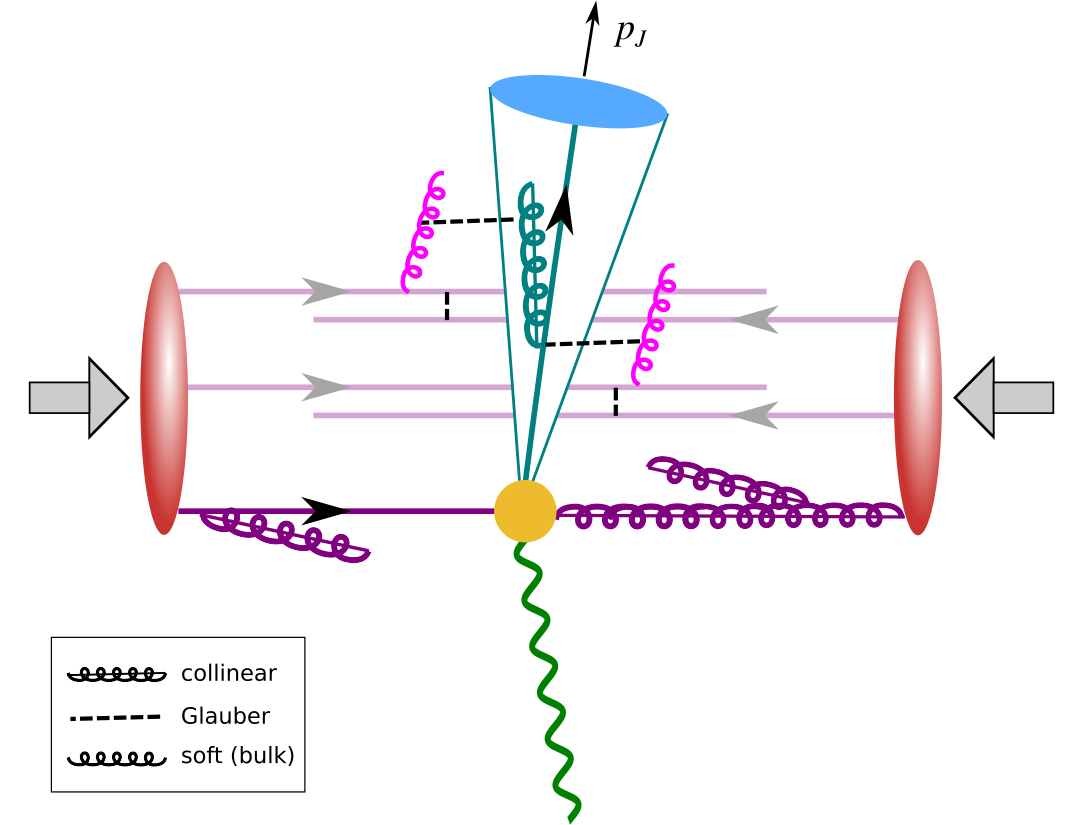
\includegraphics[width=0.65\textwidth]{fig/AA}\\
\end{center}
\vspace{2mm}
\begin{enumerate}
\item{\large There are many "good" models for jet quenching.}
\vspace{4mm}
\item{\large Differences can mostly trace back to the modelling of  bulk matter.}
\vspace{4mm}
\item{\large\bf\color{darkred} Let us take a top-down approach from QCD!}
\end{enumerate}
\end{frame}
% %
% %%%%%%%%%%%%%%%%%%%%%%%%%%%%%%%%%%%%%%%%%%%%%%%%%%%%%%%%%%
% %
% \begin{frame}{\bf\huge Everything starts from QCD on the SK contour.}	\vspace{2mm}
% \begin{enumerate}
% \item{\large Time-dependent observations are calculated in QFT on}
% \vspace{2mm}
% \begin{center}
% 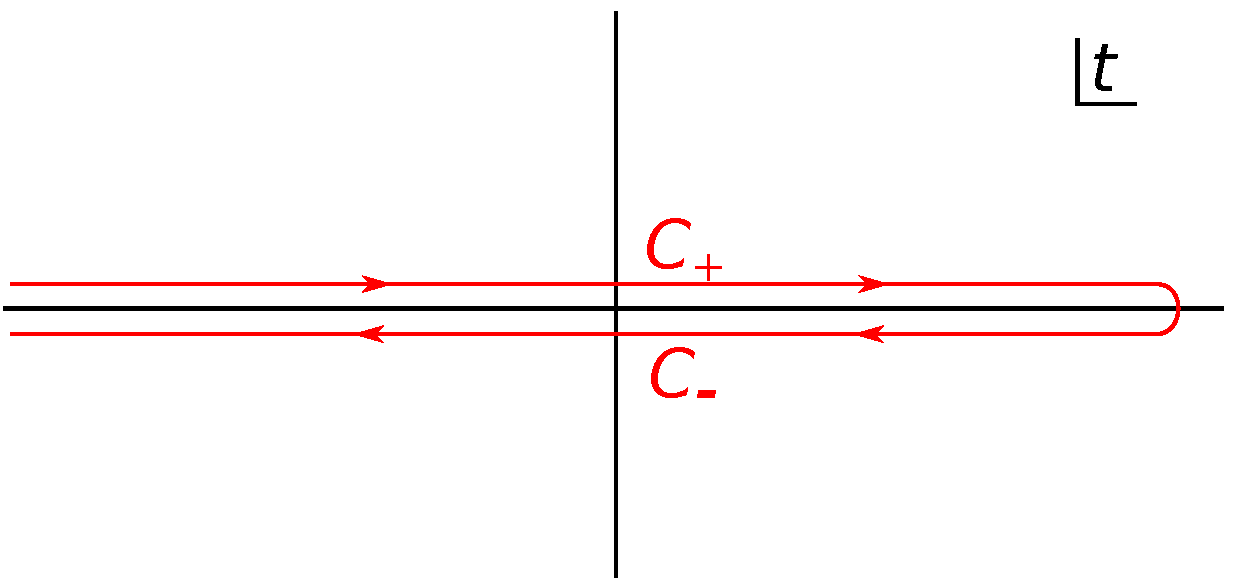
\includegraphics[width=0.65\textwidth]{fig/SKcontour}\\
% {\tiny {\color{teablue}
% Schwinger, {\emph{J.Math.Phys.} {\bfseries 2}
%   (1961) 407--432}; Keldysh,
%   {\emph{Zh.Eksp.Teor.Fiz.} {\bfseries 47} (1964) 1515--1527}.
%   }}
% \end{center}
% \vspace{2mm}
% \item{\large Equivalently, double the fields:}
% \begin{align}
%     \mathcal{L}_{QCD, I}(\phi)\to \mathcal{L}_{QCD, I}(\Phi_{+}) - \mathcal{L}_{QCD, I}(\Phi_{-})\notag
% \end{align}
% with $\Phi$ quark and gluon fields and $\Phi_\pm$ fields respectively on $C_\pm$.\\
% \begin{center}
% {\tiny For a recent discussion in QCD, see {\color{teablue}
%  Jeon, {\emph{Annals Phys.}
%   {\bfseries 340} (2014) 119--170};   BW and Kovchegov,
%   %``Time-dependent observables in heavy ion collisions. Part I. Setting up the formalism,''
%   JHEP {\bf 1803}, 158 (2018).
%   }}
% \end{center}
% \end{enumerate}
% \end{frame}

% %
% %%%%%%%%%%%%%%%%%%%%%%%%%%%%%%%%%%%%%%%%%%%%%%%%%%%%%%%%%%
% %
% \begin{frame}{\bf\huge The full problem of jet production}
% \vspace{4mm}
% \begin{center}
% 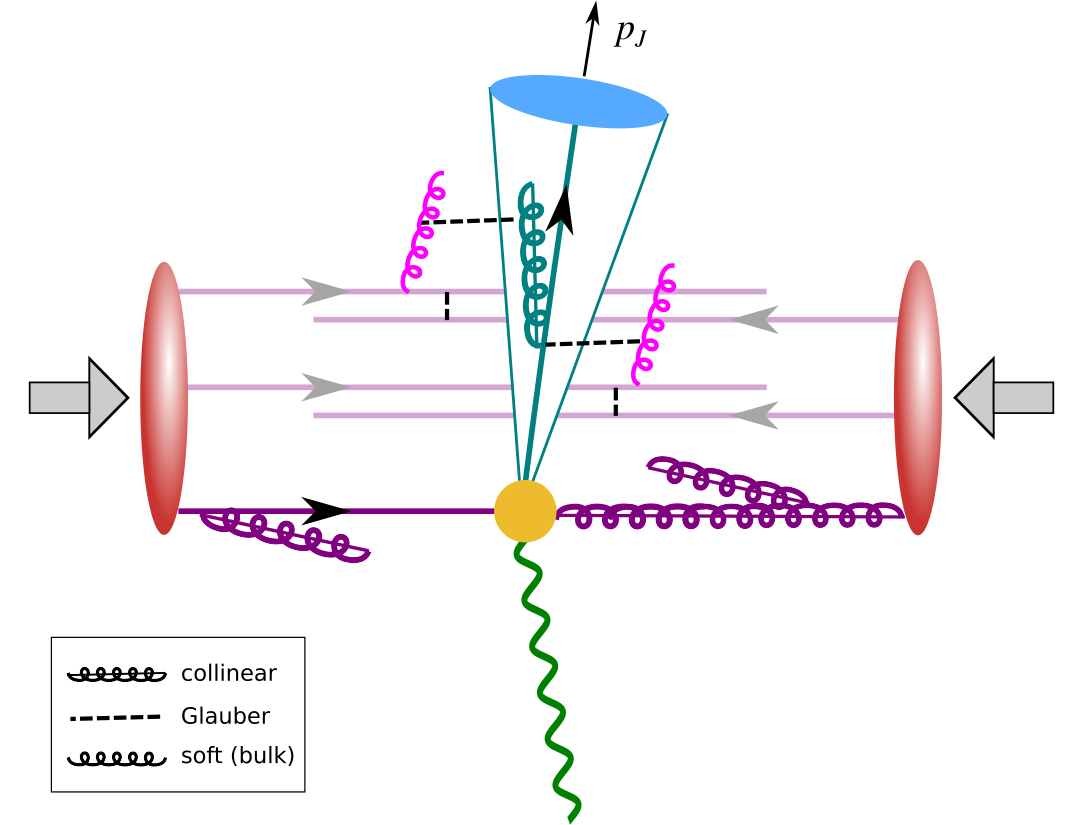
\includegraphics[width=0.6\textwidth]{fig/AA}\\
% \end{center}
% \vspace{2mm}
% {\large In jet production, we measure:}
% \begin{enumerate}
%     \item{\large Jets}
%     \item{\large Soft particles to determine centrality}
% \end{enumerate}
% \end{frame}
%
%%%%%%%%%%%%%%%%%%%%%%%%%%%%%%%%%%%%%%%%%%%%%%%%%%%%%%%%%%
%
\begin{frame}{\bf\huge Simplification: QCD Factorization}	\vspace{4mm}
\begin{center}
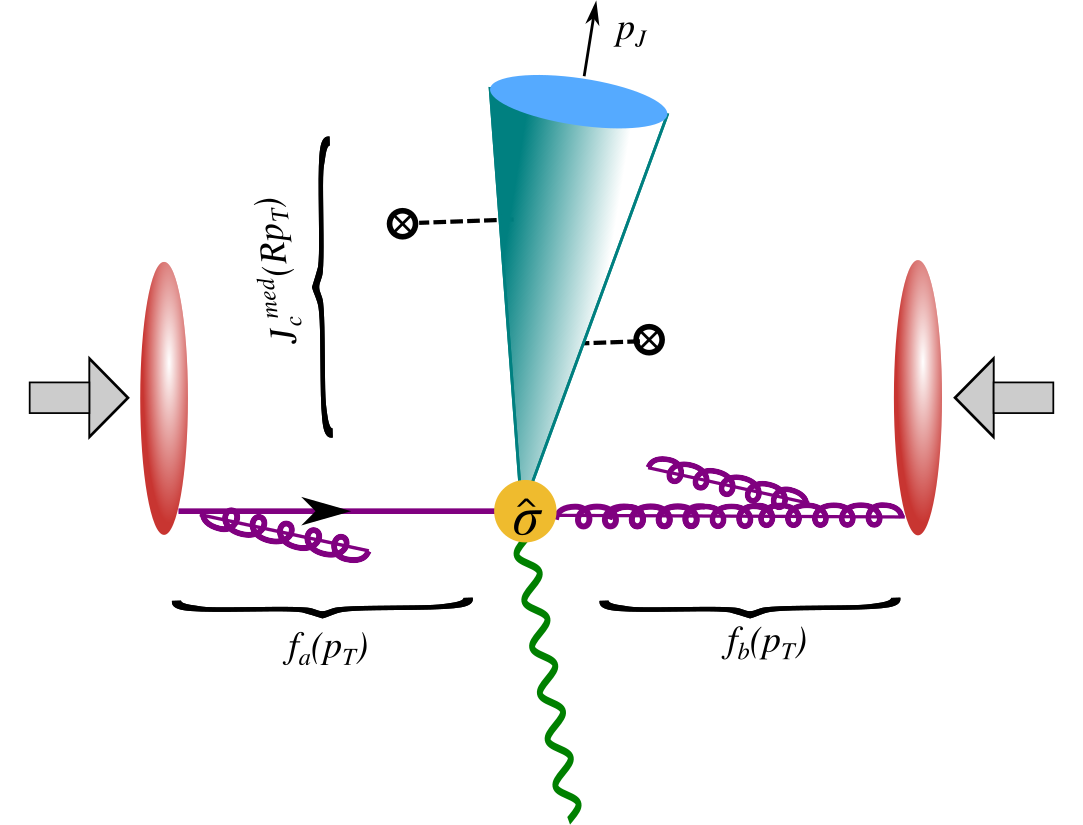
\includegraphics[width=0.6\textwidth]{fig/facotrization}\\
\end{center}
%\vspace{2mm}
\begin{enumerate}
\item{A factorization formula:}
\begin{align}
    \frac{d\sigma}{dp_{T} d\eta} =\sum\limits_{abc}f_a\otimes f_b \otimes \hat{\sigma}_{ab\to c}\otimes \underbrace{J_c^{med}}_{\text{\color{darkred}Bulk enters.}}\notag
\end{align}
\begin{center}
{\tiny  For a recent discussion: {\color{teablue}
  Qiu, Ringer, Sato and Zurita,
  %``Factorization of jet cross sections in heavy-ion collisions,''
  Phys.\ Rev.\ Lett.\  {\bf 122}, no. 25, 252301 (2019)
  %[arXiv:1903.01993 [hep-ph]]
  .
  }}\\
  \vspace{2mm}
 {\color{darkred}\bf A better understanding of bulk is need!
 %$\textcircled{1}$ a proof in QCD is still missing!
 }
\end{center}
\end{enumerate}
\end{frame}
%
%%%%%%%%%%%%%%%%%%%%%%%%%%%%%%%%%%%%%%%%%%%%%%%%%%%%%%%%%%
%
\begin{frame}{\bf\huge The Bjorken Picture}	\vspace{4mm}
\begin{center}
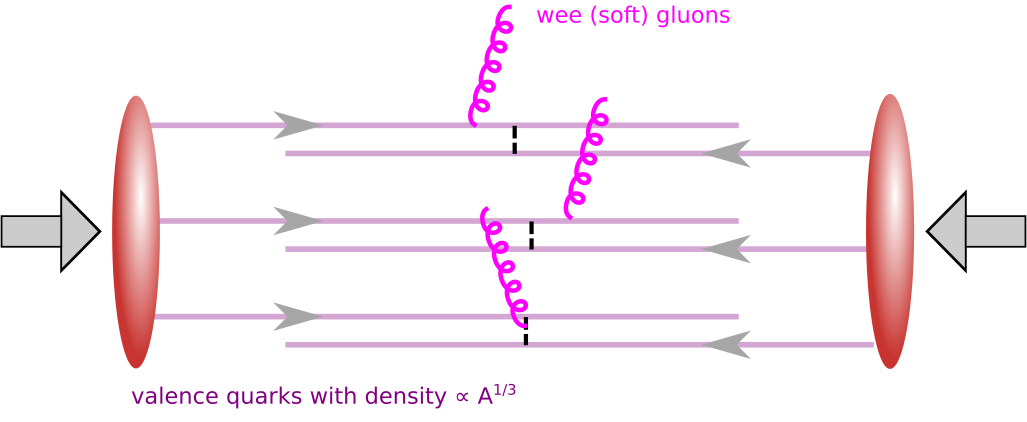
\includegraphics[width=0.65\textwidth]{fig/Bjorken}\\
{\tiny  {\color{teablue}
Bjorken,
  %``Hadron Final States in Deep Inelastic Processes,''
  Lect.\ Notes Phys.\  {\bf 56}, 93 (1976).
  }}
\end{center}
%\vspace{4mm}
% {\large How far one can go beyond such a parton picture?}
\begin{enumerate}
\item{\large The valence quarks pass through each other.}
\vspace{2mm}
\item{\large Soft ("wee") partons are freed from the wave function.}
\vspace{2mm}
\item{\large Product: a central plateau in the rapidity distribution.}\\
\vspace{1mm}
    {\color{darkred}longitudinal boost invariance} (around mid-rapidity)
\vspace{1mm}
\item{\large The saturation model (CGC): $k\sim Q_s$}
\begin{center}
    {\tiny  A comprehensive review: {\color{teablue}
  Kovchegov and Levin,
  %``Quantum chromodynamics at high energy,''
  Camb.\ Monogr.\ Part.\ Phys.\ Nucl.\ Phys.\ Cosmol.\  {\bf 33}, 1 (2012).
  %%CITATION = doi:10.1017/CBO9781139022187;%%
  %178 citations counted in INSPIRE as of 25 May 2020
.
  }}
\end{center}
\end{enumerate}
\vspace{1mm}
\begin{center}
{\bf\large\color{darkred} Let us see how far we can go from this picture?}
\end{center}
\end{frame}
% %
% %%%%%%%%%%%%%%%%%%%%%%%%%%%%%%%%%%%%%%%%%%%%%%%%%%%%%%%%%%
% %
% \setcounter{page}{0}
% \begin{frame}
% \topskip0pt
% \vspace*{\fill}
% \begin{center}
% {\Huge\bf\color{gray} Tools in our toolbox}
% \end{center}
% \vspace*{\fill}
% \end{frame}
% %
% %%%%%%%%%%%%%%%%%%%%%%%%%%%%%%%%%%%%%%%%%%%%%%%%%%%%%%%%%%
% %
% \begin{frame}{\bf\huge The Color-Glass Condensate}	\vspace{4mm}
% \begin{center}
% 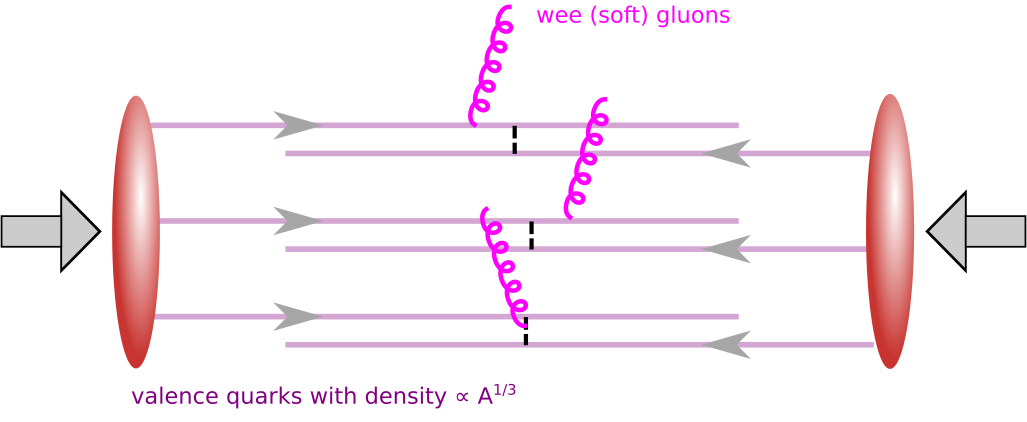
\includegraphics[width=0.65\textwidth]{fig/Bjorken}\\
% {\tiny  {\color{teablue}
% Bjorken,
%   %``Hadron Final States in Deep Inelastic Processes,''
%   Lect.\ Notes Phys.\  {\bf 56}, 93 (1976).
%   }}
% \end{center}
% %\vspace{4mm}
% \begin{enumerate}
% \item{The modern revivial: saturation physics (color-glass condensate)}\\
% \begin{center}
%     {\tiny  {\color{teablue}
%   Kovchegov and Levin,
%   %``Quantum chromodynamics at high energy,''
%   Camb.\ Monogr.\ Part.\ Phys.\ Nucl.\ Phys.\ Cosmol.\  {\bf 33}, 1 (2012).
%   %%CITATION = doi:10.1017/CBO9781139022187;%%
%   %178 citations counted in INSPIRE as of 25 May 2020
% .
%   }}
% \end{center}
% \item{The longitudinal boost-invariance:}\\
% \vspace{1mm}
% {\small For example, at $O(\alpha_s A^{2/3})$ and large $\tau$}
% \begin{align}
%   f^{cl}(X,p)=\frac{1}{\tau} \theta(X^+) \theta(X^-) \delta(y-\eta)
%   f_\perp^{cl}(\underline{p})
%   \notag
% \end{align}
% with
% $f_\perp^{cl}(\underline{p})\equiv\frac{8\pi^2\alpha_s^3}{N_c}\left(\frac{A}{S_\perp}\right)^2
%   \frac{1}{p_T^5}\ln\left(\frac{p_T^2}{\Lambda^2}\right).$
% \begin{center}
%     {\tiny  {\color{teablue}
% \bibitem{Wu:2017rry} 
%   BW and Kovchegov,
%   %``Time-dependent observables in heavy ion collisions. Part I. Setting up the formalism,''
%   JHEP {\bf 1803}, 158 (2018)
%   [arXiv:1709.02866 [hep-ph]].
% }}
% \end{center}
% \end{enumerate}
% \end{frame}
%
%%%%%%%%%%%%%%%%%%%%%%%%%%%%%%%%%%%%%%%%%%%%%%%%%%%%%%%%%%
%https://www.overleaf.com/project/5ec7eb5acba0510001502bd9
\setcounter{page}{0}
\begin{frame}
\topskip0pt
\vspace*{\fill}
\begin{center}
{\Huge\bf\color{gray} Bulk in AA collisions}
\end{center}
\vspace*{\fill}
\end{frame}
%
%%%%%%%%%%%%%%%%%%%%%%%%%%%%%%%%%%%%%%%%%%%%%%%%%%%%%%%%%%
%
\setcounter{page}{4}
\begin{frame}{\bf\huge The Bottom-up Thermalization}	\vspace{2mm}
\begin{center}
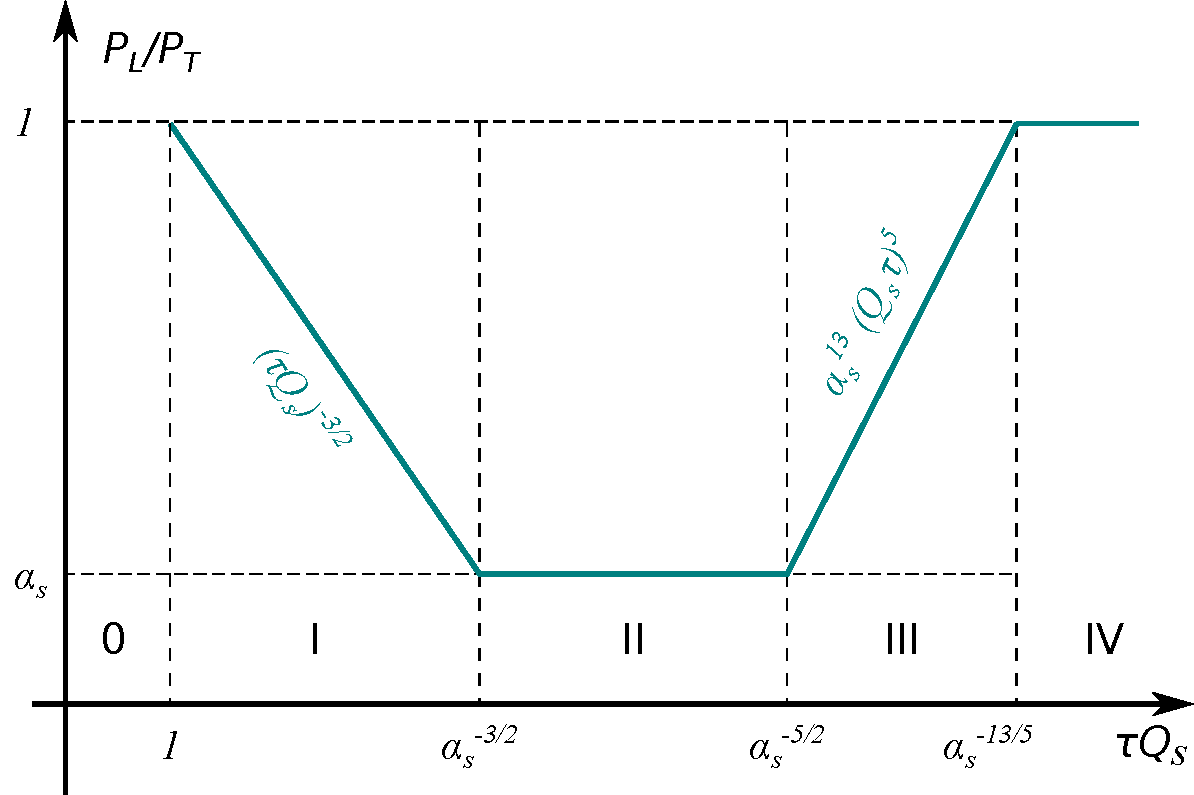
\includegraphics[width=0.6\textwidth]{fig/PLoPT}\\
\vspace{4mm}
% \begin{tabular}{ c|| c c c c c c}
% \hline
% time interval& hard $f$ & soft $f$&$\frac{N_h}{Q_s^3}$ & $\frac{N_s}{Q_s^3}$ & $\frac{\epsilon}{Q_s^4}$ & $\frac{P_L}{P_T}$\\
% \hline\hline
%  $ \alpha_s^{-\frac{3}{2}}> \tau Q_s > 1$ &$\frac{1}{\alpha_{s} (\tau Q_s)^{\frac{2}{3}}}$ & $\frac{1}{\alpha_{s} (\tau Q_s)^{\frac{1}{3}}}$ & $\frac{1}{\alpha_s \tau Q_s}$ & $\frac{1}{\alpha_s (\tau Q_s)^{\frac{4}{3}}}$ & $\frac{1}{\alpha_s \tau Q_s}$ & $\frac{1}{(\tau Q_s)^{\frac{2}{3}}}$\\
%  \hline
%  $ \alpha_s^{-\frac{5}{2}}> \tau Q_s > \alpha_s^{-\frac{3}{2}}$ &$\frac{1}{\alpha_{s}^{\frac{3}{2}} \tau Q_{s} }$ & $\frac{1}{\alpha_{s}^{\frac{5}{4}} (\tau Q_s)^{\frac{1}{2}}}$ & $\frac{1}{\alpha_s \tau Q_s}$ & $\frac{ \alpha_{s}^{\frac{1}{4}}}{(\tau Q_s)^{\frac{1}{2}}}\right]$$ & $\frac{1}{\alpha_s \tau Q_s}$ & $\alpha_s$\\
%   \hline
%  $ \alpha_s^{-\frac{13}{5}}> \tau Q_s > \alpha_s^{-\frac{5}{2}}$ &$\frac{1}{\alpha_{s} (\tau Q_s)^{\frac{2}{3}}}$ & $\frac{1}{\alpha_{s} (\tau Q_s)^{\frac{1}{3}}}$ & $\frac{1}{\alpha_s \tau Q_s}$ & $\frac{1}{\alpha_s (\tau Q_s)^{\frac{4}{3}}}$ & $\frac{1}{\alpha_s \tau Q_s}$ & $ \alpha_{s}^{13} (\tau Q_s)^{5}$\\
%  %$ \alpha_s^{-\frac{5}{2}}> \tau Q_s > \alpha_s^{-\frac{3}{2}}$ & cell5 & cell6 \\  
%  %cell7 & cell8 & cell9    
%  \hline
% \end{tabular}\\
\begin{tabular}{ l|| c c c c c c}
\hline
stage&$N_s/N_h$ & $\epsilon_s/Q_s^4$ & $\tau/\tau_{th}$ & $T$\\
\hline\hline
 I: $\alpha_s^{-\frac{3}{2}}> \tau Q_s > 1$ 
 & $(\tau Q_s)^{-\frac{1}{3}}$ 
 & $\alpha_{s}^{-1} (\tau Q_s)^{-\frac{5}{3}}$
 & $\alpha_{s}^{\frac{7}{4}} (\tau Q_s)^{\frac{7}{12}}$
 &0\\
 \hline
 II: $\alpha_s^{-\frac{5}{2}}> \tau Q_s > \alpha_s^{-\frac{3}{2}}$ 
 & $\alpha_{s}^{\frac{5}{4}} (\tau Q_s)^{\frac{1}{2}}$
 & $\alpha_{s}^{\frac{3}{4}}(\tau Q_s)^{-\frac{1}{2}}$
 & $\alpha_{s}^{\frac{35}{16}} (\tau Q_s)^{\frac{7}{8}}$
 &0\\
  \hline
 III: $\alpha_s^{-\frac{13}{5}}> \tau Q_s > \alpha_s^{-\frac{5}{2}}$ 
 & $\alpha_{s}^{10} (\tau Q_s)^{4}$
 & $\alpha_{s}^{12} (\tau Q_s)^{4}$ 
 & $ \alpha_{s}^{5} (\tau Q_s)^{2}$
 & $ \alpha_{s}^{3} Q_{s}^{2} \tau$\\
 %$ \alpha_s^{-\frac{5}{2}}> \tau Q_s > \alpha_s^{-\frac{3}{2}}$ & cell5 & cell6 \\  
 %cell7 & cell8 & cell9    
 \hline
\end{tabular}\\
\vspace{2mm}
{\small Note that $N_h \sim Q_s^2/(\alpha_s\tau)$ and $\epsilon_h\sim Q_s N_h$.}\\
\vspace{2mm}
    {\tiny  {\color{teablue}
  Baier, Mueller, Schiff and Son,
  %``'Bottom up' thermalization in heavy ion collisions,''
  Phys.\ Lett.\ B {\bf 502}, 51 (2001)
  [hep-ph/0009237].
}}
\end{center}
\end{frame}
%
%%%%%%%%%%%%%%%%%%%%%%%%%%%%%%%%%%%%%%%%%%%%%%%%%%%%%%%%%%
%
\begin{frame}{\bf\huge Stage 0: free soft gluon from wave functions}
\begin{center}
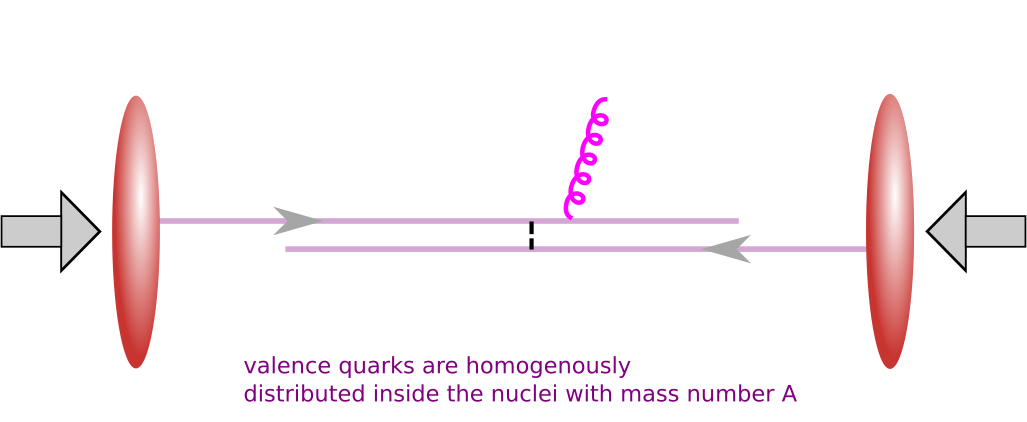
\includegraphics[width=0.55\textwidth]{fig/classical}\\
\end{center}
\begin{enumerate}
\item{\large\bf Energy density:} $\epsilon\propto \frac{1}{\tau}~\text{at large $\tau$}$\\
\vspace{1mm}
\begin{center}
{\tiny  {\color{teablue}
  Kovchegov,
  %``Can thermalization in heavy ion collisions be described by QCD diagrams?,''
  Nucl.\ Phys.\ A {\bf 762}, 298 (2005)
  [hep-ph/0503038];
  Lappi,
  %``Energy density of the glasma,''
  Phys.\ Lett.\ B {\bf 643}, 11 (2006)
  [hep-ph/0606207].
}}
\end{center}
\vspace{1mm}
\item{\large\bf Two point function in the limit $\tau\to\infty$}
\begin{align}
G_{22}^{a\mu,b\nu}(X, p) \to  2\pi\delta(p^2) \delta^{ab}
  \sum\limits_{\lambda=\pm}\epsilon_\lambda^\mu(p)
  \epsilon_{\lambda}^{*\nu}(p) f^{cl}(X,p)\notag
\end{align}
where $f^{cl}(X,p)=\frac{1}{\tau} \theta(X^+) \theta(X^-) \delta(y-\eta)
  f_\perp^{cl}(\underline{p})$\\
with $y = \frac{1}{2}\ln\frac{p^+}{p^-}$, $\eta = \frac{1}{2}\ln\frac{X^+}{X^-}$ and
$f_\perp^{cl}(\underline{p})\equiv\frac{8\pi^2\alpha_s^3}{N_c}\left(\frac{A}{S_\perp}\right)^2
  \frac{1}{p_T^5}\ln\left(\frac{p_T^2}{\Lambda^2}\right).$
  \vspace{1mm}

\begin{center}
  {\bf \color{darkred}\bf$\delta(p^2)$: classical field does go on mass-shell as $\tau\to\infty$!}\\
  \vspace{1mm}
  {\tiny  {\color{teablue}
  BW and Kovchegov,
  %``Time-dependent observables in heavy ion collisions. Part I. Setting unp the formalism,''
  JHEP {\bf 1803}, 158 (2018)
  [arXiv:1709.02866 [hep-ph]].
}}
\end{center}
\end{enumerate}
\end{frame}
%
%%%%%%%%%%%%%%%%%%%%%%%%%%%%%%%%%%%%%%%%%%%%%%%%%%%%%%%%%%
%
\begin{frame}{\bf\huge From classical fields to Boltzmann equation?}\\
\vspace{1mm}
{\large\bf The question:}
\begin{align}
f^{(1)}=\sum\begin{array}{c}
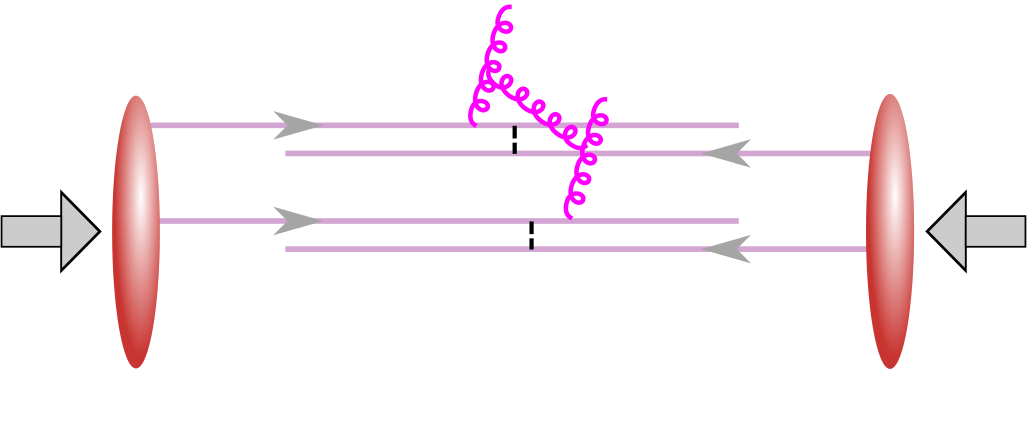
\includegraphics[width=0.55\textwidth]{fig/CF2BE}
\end{array}\notag
\end{align}
with $f^{(1)}$ solved from $\left(\frac{\partial}{\partial t} - \frac{1}{t} p_z
    \frac{\partial}{\partial p_z}\right)
  f^{(1)}= C_{2\leftrightarrow2}[f^{cl}]$.\\
\vspace{2mm}
{\large\bf The result:}
\begin{enumerate}
    \item {\large They are the same only if certain approximations imposed.}
\begin{center}
 {\tiny  {\color{teablue}
  BW and Kovchegov,
  %``Time-dependent observables in heavy ion collisions. Part I. Setting unp the formalism,''
  JHEP {\bf 1803}, 158 (2018)
  [arXiv:1709.02866 [hep-ph]].
}}
\end{center}
    \item {\large A detailed calculation in $\phi^4$ theory shows otherwise.}
\begin{center}
 {\tiny  {\color{teablue}
  Kovchegov and BW,
  %``Time-dependent observables in heavy ion collisions. Part II. In search of pressure isotropization in the $\varphi^4$ theory,''
  JHEP {\bf 1803}, 157 (2018)
  [arXiv:1709.02868 [hep-ph]].
}}\\\vspace{2mm}
{\bf \color{red} Yet to be understood in QCD!}
\end{center}
\end{enumerate}
\end{frame}
%
%%%%%%%%%%%%%%%%%%%%%%%%%%%%%%%%%%%%%%%%%%%%%%%%%%%%%%%%%%
%
\begin{frame}{\bf\huge Some detailed simulations}	\vspace{2mm}
{\large \bf Confirmation of Bottom-up thermalization:}\\
\vspace{2mm}
\begin{enumerate}
    \item {\large Stage I from classical statistical approximation (CSA):}
\begin{center}
    {\tiny  {\color{teablue}
  Berges, Boguslavski, Schlichting and Venugopalan,
  %``Universal attractor in a highly occupied non-Abelian plasma,''
  Phys.\ Rev.\ D {\bf 89}, 114007 (2014)
  [arXiv:1311.3005 [hep-ph]].
}}
\end{center}
    \item {\large Bottom-up in kinetic theory:}
\begin{center}
    {\tiny  {\color{teablue}
  Kurkela and Zhu,
  %``Isotropization and hydrodynamization in weakly coupled heavy-ion collisions,''
  Phys.\ Rev.\ Lett.\  {\bf 115}, 182301 (2015)
  [arXiv:1506.06647 [hep-ph]].
}}
\end{center}
    \item {\large An entire evolution by matching:}
\begin{center}
    {\tiny  {\color{teablue}
  Kurkela, Mazeliauskas, Paquet, Schlichting and Teaney,
  %``Matching the Nonequilibrium Initial Stage of Heavy Ion Collisions to Hydrodynamics with QCD Kinetic Theory,''
  Phys.\ Rev.\ Lett.\  {\bf 122}, 122302 (2019)
  [arXiv:1805.01604 [hep-ph]].
}}
\end{center} 
\end{enumerate}
\vspace{2mm}
{\large \bf Beyond "purely" classical limit in CSA:}\\
\begin{enumerate}
\vspace{1mm}
    \item {\large Method:}\\
    \vspace{1mm}
    The vacuum (quantum) fluctuation is included in the initial condition.
    \item{\large {\bf Prons:} Fast isotripization has been shown in CSA.}
    \begin{center}
    {\tiny  {\color{teablue}
  Epelbaum and Gelis,
  %``Pressure isotropization in high energy heavy ion collisions,''
  Phys.\ Rev.\ Lett.\  {\bf 111}, 232301 (2013)
  [arXiv:1307.2214 [hep-ph]].
}}
\end{center} 
    \item{\large {\bf Cons:} One has to deal with nonrenormalizablity}
        \begin{center}
    {\tiny  {\color{teablue}
  Epelbaum, Gelis and BW,
  %``Nonrenormalizability of the classical statistical approximation,''
  Phys.\ Rev.\ D {\bf 90}, no. 6, 065029 (2014)
  [arXiv:1402.0115 [hep-ph]].\\
    Berges, Boguslavski, Schlichting and Venugopalan,
  %``Basin of attraction for turbulent thermalization and the range of validity of classical-statistical simulations,''
  JHEP {\bf 1405}, 054 (2014)
  [arXiv:1312.5216 [hep-ph]].
}}
\end{center} 
\end{enumerate}

\end{frame}
%
%%%%%%%%%%%%%%%%%%%%%%%%%%%%%%%%%%%%%%%%%%%%%%%%%%%%%%%%%%
%
\begin{frame}{\bf\huge Connection to jet quenching}	\vspace{2mm}
\begin{center}
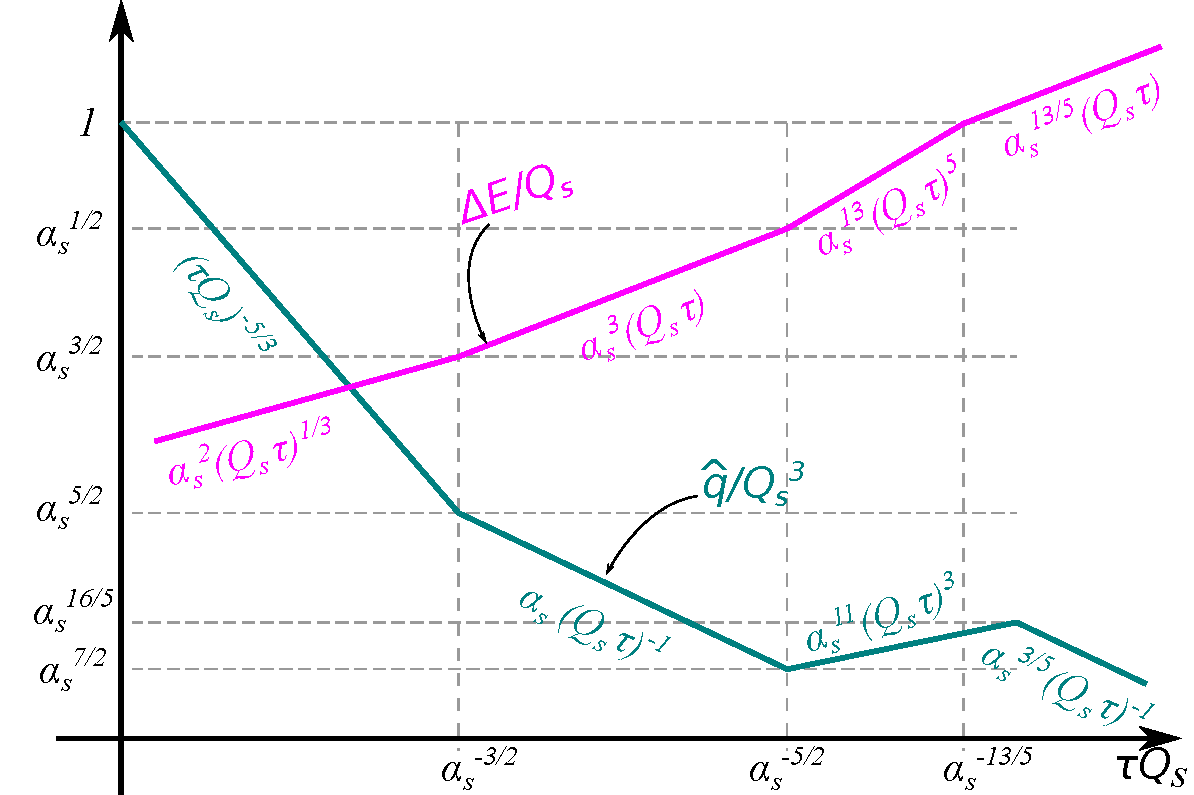
\includegraphics[width=0.8\textwidth]{fig/qhatInBottomUp}
\end{center}
\end{frame}
%
%%%%%%%%%%%%%%%%%%%%%%%%%%%%%%%%%%%%%%%%%%%%%%%%%%%%%%%%%%
%
\begin{frame}{\bf\huge Connection to jet quenching}	\vspace{2mm}
{\large\bf Some detailed calculations:}
\vspace{2mm}
\begin{enumerate}
    \item{\large Radiative energy spectrum can be calculated analysitcally.}
    \begin{align}
        \omega\frac{dI}{d\omega} \sim \alpha_s N_c \sqrt{\frac{\hat{q}(\tau)\tau^2}{\omega}}
        \qquad\text{for $t_f \ll \tau$}\notag
    \end{align}
\begin{center}
    {\tiny  {\color{teablue}
  Baier, Dokshitzer, Mueller and Schiff,
  %``Radiative energy loss of high-energy partons traversing an expanding QCD plasma,''
  Phys.\ Rev.\ C {\bf 58}, 1706 (1998); Arnold,
  %``Simple Formula for High-Energy Gluon Bremsstrahlung in a Finite, Expanding Medium,''
  Phys.\ Rev.\ D {\bf 79}, 065025 (2009).
}}    
\end{center}
\vspace{2mm}
    \item{\large Radiative correction to $p_T$-broadening and $\hat{q}$:}\\
    \vspace{2mm}
    \begin{itemize}
        \item{Leading-log and resummation}
        \begin{align}
        \hat{q}_{resum}(\tau) = \hat{q}(\tau)\,
        \frac{\rmI_1\big(2 \sqrt{\abar}\, Y\big)}{\sqrt{\abar}\,Y}\qquad\text{with $Y=\ln(\tau/\lambda(\tau))$}\notag
        \end{align}
        looks like a static medium with $\hat{q} = \hat{q}(\tau)$ at each time!\\
\begin{center}
    {\tiny  {\color{teablue}
  Iancu, Taels and BW,
  %``Jet quenching parameter in an expanding QCD plasma,''
  Phys.\ Lett.\ B {\bf 786}, 288 (2018)
  [arXiv:1806.07177 [hep-ph]].
  }}
\end{center}
    \vspace{2mm}
        \item{Finite terms may also be important: {\tiny  {\color{teablue}
  Zakharov,
  %``Radiative $p_{\perp}$-broadening of fast partons in an expanding quark-gluon plasma,''
  arXiv:2003.10182 [hep-ph].
  %%CITATION = ARXIV:2003.10182;%%
}}
}
    \end{itemize}
\end{enumerate}
\end{frame}
%
%%%%%%%%%%%%%%%%%%%%%%%%%%%%%%%%%%%%%%%%%%%%%%%%%%%%%%%%%%
%
\setcounter{page}{0}
\begin{frame}
\topskip0pt
\vspace*{\fill}
\begin{center}
{\Huge\bf\color{gray} Bulk in small systems}
\end{center}
\vspace*{\fill}
\end{frame}


%
%
%%%%%%%%%%%%%%%%%%%%%%%%%%%%%%%%%%%%%%%%%%%%%%%%%%%%%%%%%%
%
\setcounter{page}{12}
\begin{frame}{\bf\huge Hydro vs Non-hydro Modes}
\vspace{4mm}
\begin{enumerate}
\item{\Large{\bf Hydrodynamics:} hydro pole of $G_R^{\alpha\beta, \gamma\delta}$}
\vspace{2mm}
\begin{columns}
\begin{column}{0.55\textwidth}
\vspace{4mm}
\begin{enumerate}
\item{\large All QFTs contain hydro.}
\vspace{4mm}
\item{\color{darkred}\large They differ in non-hydro.}
\end{enumerate}
\vspace{4mm}
\end{column}
\begin{column}{0.3\textwidth}
%\setcounter{page}{2}
\begin{center}
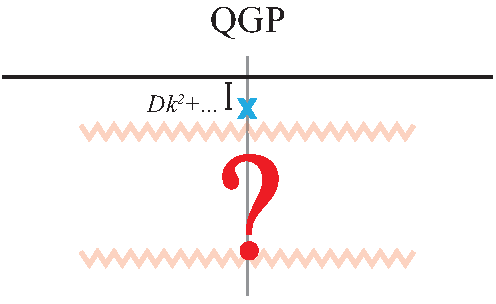
\includegraphics[width=\textwidth]{fig/omega_QCD}
\end{center}
\end{column}
\end{columns}
\vspace{4mm}
\begin{center}
the analytic structure of {\small $G_R^{\alpha\beta, \gamma\delta}(\omega, \vec{k}) = -i\int d^4 x e^{ik\cdot x}\theta(x^0)\langle[T^{\alpha\beta}(x),T^{\gamma\delta}(0)] \rangle$}
\\\vspace{1mm}
{\tiny  For a review: {\color{teablue}
  Florkowski, Heller and Spalinski,
  %``New theories of relativistic hydrodynamics in the LHC era,''
  Rept.\ Prog.\ Phys.\  {\bf 81}, no. 4, 046001 (2018)
  [arXiv:1707.02282 [hep-ph]].
  }}
\end{center}
\item{\large{\bf Hydrodynamic models}: hydro + some non-hydro modes}
\vspace{2mm}
\begin{enumerate}
    \item{\large The Israel-Stewart (IS) hydro:}
    \begin{center}
    {\tiny {\color{teablue}
    Israel and Stewart,
  %``Transient relativistic thermodynamics and kinetic theory,''
  Annals Phys.\  {\bf 118}, 341 (1979)..
    }}
\end{center}
\item{$\cdots$}
\end{enumerate}
\item{\large \bf Condition for applicability of hydrodynamic models:}\\
\begin{center}
   {\bf \color{darkred} hydro modes dominate non-hydro modes}
\end{center}
\end{enumerate}
\end{frame}
% %
% %%%%%%%%%%%%%%%%%%%%%%%%%%%%%%%%%%%%%%%%%%%%%%%%%%%%%%%%%%
% %
% \begin{frame}{\bf\huge IS Hydro Is Not Only Hydro}
% \vspace{4mm}
% \begin{center}
% 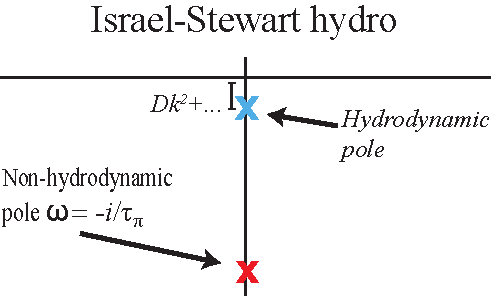
\includegraphics[width=0.6\textwidth]{fig/omega_IS}
% \end{center}
% {\tiny {\color{white} Romatschke,
%   %``Retarded correlators in kinetic theory: branch cuts, poles and hydrodynamic onset transitions,''
%   Eur.\ Phys.\ J.\ C {\bf 76}, no. 6, 352 (2016)
%   %doi:10.1140/epjc/s10052-016-4169-7
%   [arXiv:1512.02641];\\Kurkela and Wiedemann,
%   %``Analytic structure of nonhydrodynamic modes in kinetic theory,''
%   arXiv:1712.04376.
%   }
%   }\vspace{4mm}\\
% %\phantom
% {{\LARGE\bf\color{darkred} The Israel-Stewart (IS) hydro}}
% %\setcounter{page}{5}
% \vspace{4mm}
% \begin{center}
% %\phantom
% {$D\Pi^{\mu\nu}+\frac{4}{3}\Pi^{\mu\nu}\nabla_\alpha u^\alpha = \frac{1}{\tau_\pi}\left(\Pi^{\mu\nu}+2 \eta\sigma^{\mu\nu}\right).$}
% \end{center}
%  \end{frame}
%
%
%%%%%%%%%%%%%%%%%%%%%%%%%%%%%%%%%%%%%%%%%%%%%%%%%%%%%%%%%%
%
\begin{frame}{\bf\huge Opportunities for studying small systems}
\vspace{4mm}
{\bf \large Two opposite directions:}
\vspace{2mm}
\begin{enumerate}
\item{\large One fluid to rule them all.}
\begin{center}
{\tiny Quotes from the title of {\color{teablue}
  Weller and Romatschke,
  %``One fluid to rule them all: viscous hydrodynamic description of event-by-event central p+p, p+Pb and Pb+Pb collisions at $\sqrt{s}=5.02$ TeV,''
  Phys.\ Lett.\ B {\bf 774}, 351 (2017)
  [arXiv:1701.07145 [nucl-th]].
}}
\end{center}
\vspace{2mm}
\item{\large\bf \color{darkred} Golden opportunity to study non-hydro modes}
\vspace{2mm}
\begin{center}
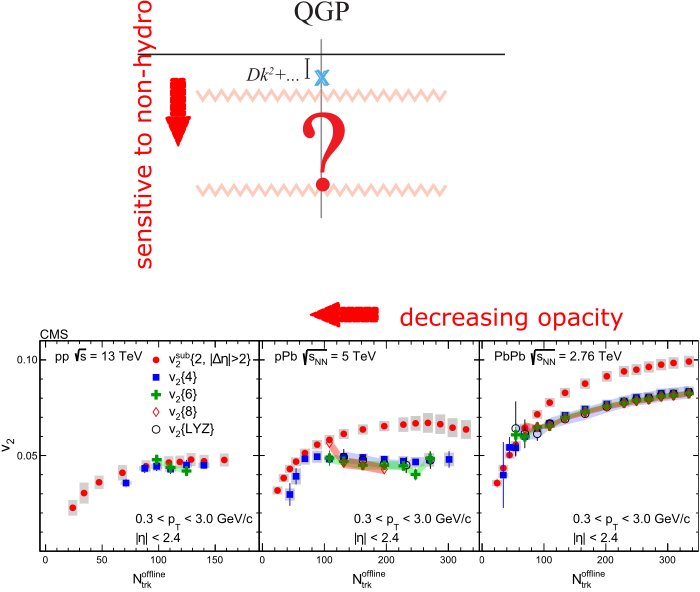
\includegraphics[width=0.6\textwidth]{fig/goal}
\vspace{2mm}\\
{\color{white}\bf\LARGE Decreasing $R\sim 1/k$ enhances non-hydro contributions.}
\end{center}
\end{enumerate}
\end{frame}
%
%%%%%%%%%%%%%%%%%%%%%%%%%%%%%%%%%%%%%%%%%%%%%%%%%%%%%%%%%%
%
\begin{frame}{\bf\huge Flow in small and/or dilute limit}
\vspace{4mm}
\begin{center}
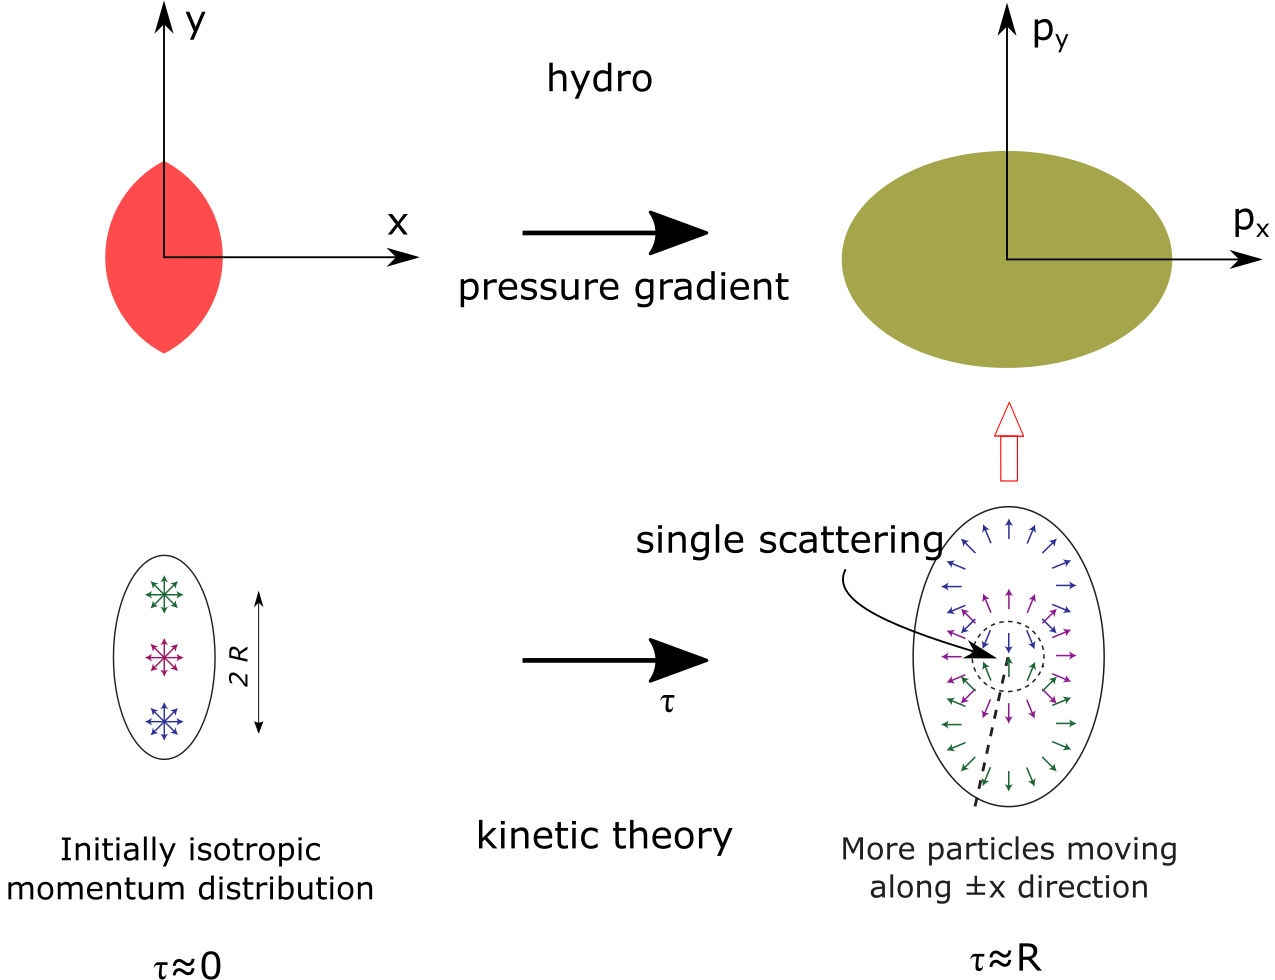
\includegraphics[width=0.65\textwidth]{fig/onehit}\\
{\tiny  {\color{teablue} Kurkela, Wiedemann and BW,
  %``Kinetic transport is needed to reliably extract shear viscosity from pA and AA data,''
  Phys.\ Lett.\ B {\bf 783}, 274 (2018), [arXiv:1803.02072].
  }
  }
\end{center}
\vspace{4mm}
{{\LARGE\color{darkred} Flow is a signature for final-state interactions, not for hydro!}}
\vspace{2mm}\\
{\tiny  See also: {\color{teablue}   Borghini \& Gombeaud,
  %``Anisotropic flow far from equilibrium,''
  Eur.\ Phys.\ J.\ C {\bf 71} (2011) 1612; He, Edmonds, Lin, Liu, Molnar \& Wang,
  %``Anisotropic parton escape is the dominant source of azimuthal anisotropy in transport models,''
  Phys.\ Lett.\ B {\bf 753} (2016) 506.
  }
}
\end{frame}
%
%
%%%%%%%%%%%%%%%%%%%%%%%%%%%%%%%%%%%%%%%%%%%%%%%%%%%%%%%%%%
%
\begin{frame}{\bf\huge Features of the early-time dynamics}
%%\setcounter{page}{6}
\vspace{2mm}
\begin{center}
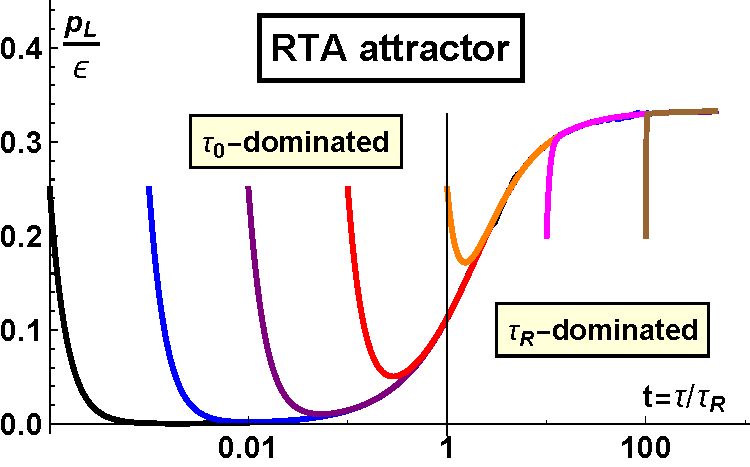
\includegraphics[width=0.4\textwidth]{fig/RTAattract}
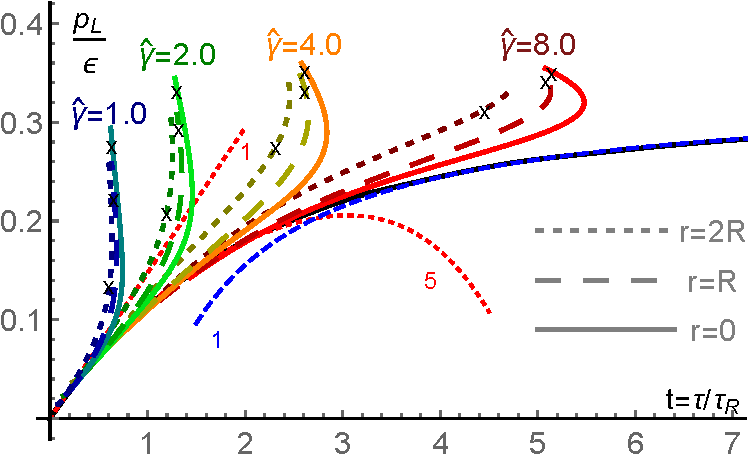
\includegraphics[width=0.4\textwidth]{fig/rcurve}\\
\vspace{2mm}
{\tiny  {\color{teablue}   Kurkela, van der Schee, Wiedemann and BW,
  %``Early- and Late-Time Behavior of Attractors in Heavy-Ion Collisions,''
  Phys.\ Rev.\ Lett.\  {\bf 124}, 102301 (2020)
  [arXiv:1907.08101 [hep-ph]]..
  }}\\
  \vspace{2mm}
  {\color{teablue} (cf. talk by Wilke van der Schee)}
\end{center}
%\phantom
\begin{enumerate}
\item{\large\bf There are some qualitative similarities to QCD.}\\
\vspace{2mm}
\begin{itemize}
\item{\large Early-time attractor}\vspace{1mm}
\item{\large Late-time (hydro) attractor}
\begin{center}
{\tiny  See, e.g., {\color{teablue}  
    Romatschke,
  %``Relativistic Fluid Dynamics Far From Local Equilibrium,''
  Phys.\ Rev.\ Lett.\  {\bf 120}, no. 1, 012301 (2018)
  [arXiv:1704.08699 [hep-th]].
  }}
\end{center}
\end{itemize}
\vspace{1mm}
\item{\bf The early-time dynamics may be modified by system size (opacity).}
\end{enumerate}
\end{frame}
%
%%%%%%%%%%%%%%%%%%%%%%%%%%%%%%%%%%%%%%%%%%%%%%%%%%%%%%%%%%
%
\begin{frame}{\bf\huge $v_2$ from Free-streaming to Ideal Hydro}
\begin{center}
\begin{overpic}[width=0.7\textwidth]{fig/ckthydrofull}
%\put (25, 46){\color{darkred}$G_R(t, k)\sim c_{hyd} e^{-D k^2 t} + \text{non-hydro terms}$}
\end{overpic}\vspace{4mm}\\
{\color{darkred}\bf\LARGE Non-hydro modes are more efficient to build up $v_2$ in small systems!}
\vspace{4mm}\\
{\tiny  {\color{teablue} Kurkela, Wiedemann and BW,
  %``Kinetic transport is needed to reliably extract shear viscosity from pA and AA data,''
  arXiv:1805.04081.
  }
  }
\end{center}
\end{frame}
%
%
%%%%%%%%%%%%%%%%%%%%%%%%%%%%%%%%%%%%%%%%%%%%%%%%%%%%%%%%%%
%

\begin{frame}{\bf\huge Qualification of Being a Fluid}
%\setcounter{page}{6}
\vspace{4mm}
{\color{darkred}\bf\LARGE Criteria:}
\vspace{4mm}
\begin{center}
{\huge\color{darkred}
\framebox[0.5\textwidth]{hydro-like $\Leftrightarrow Q<0.1$}
}
\end{center}
\vspace{4mm}
{\Large \color{black} in terms of  ''fluid quality''}
\begin{center}
{\Large\color{black}
%\framebox[1.1\width]
{
$Q(t,r) =  \sqrt{  \frac{ \left( T_{\rm kin}- T_{\rm hyd} \right)^{\mu\nu}   \left( T_{\rm kin} - T_{\rm hyd} \right)_{\mu\nu} }{ \left(T_{\rm id} \right)^{\mu\nu}    \left(T_{\rm id} \right)_{\mu\nu}    }  }.$
}
}
\vspace{2mm}\\
{\tiny  {\color{teablue} Kurkela, Wiedemann and BW, arXiv:1905.05139.
%doi:10.1088/1126-6708/2008/04/100
%[arXiv:0712.2451].
  }
  }
\end{center}
\vspace{2mm}
{\color{black}\Large Up to 2nd order in gradient expansion, }
\begin{align}
&T_{\rm hyd}^{\mu\nu} = \left( \varepsilon + p\right) u^\mu\, u^\nu + p\, g^{\mu\nu} + \Pi^{\mu\nu}_{\rm hyd}\nonumber\\
&\Pi^{\mu\nu}_{\rm hyd} = - 2 \eta \sigma^{\mu\nu}+ 2 \tau_{\Pi}\, \eta \left[ ^<D\sigma^{\mu\nu>} 
	+ \frac{1}{3} \sigma^{\mu\nu} \nabla_\alpha u^\alpha \right] +	\lambda_1 \sigma^{<\mu}_\alpha\, \sigma^{\nu> \lambda} \nonumber\\
&\sigma^{\mu\nu} =  \left\{\frac{1}{2}\left[ \Delta^{\mu\alpha} \nabla_\alpha u^\nu {+} \Delta^{\nu\alpha} \nabla_\alpha u^\mu \right] 
				{-} \frac{1}{3}\Delta^{\mu\nu} \nabla_\alpha u^\alpha \right\}\nonumber
\end{align}
\begin{center}
\vspace{2mm}
{\tiny  {\color{teablue}   Baier, Romatschke, Son, Starinets and Stephanov,
  %``Relativistic viscous hydrodynamics, conformal invariance, and holography,''
  JHEP {\bf 0804}, 100 (2008).
%doi:10.1088/1126-6708/2008/04/100
%[arXiv:0712.2451].
  }
  }
  \end{center}
\end{frame}
%
%%%%%%%%%%%%%%%%%%%%%%%%%%%%%%%%%%%%%%%%%%%%%%%%%%%%%%%%%%
%
\begin{frame}{\bf\huge How Much "Fluid" is CKT?}
\vspace{4mm}
\begin{center}
\begin{overpic}[width=1\textwidth]{fig/Q1}
%\put (25, 46){\color{darkred}$G_R(t, k)\sim c_{hyd} e^{-D k^2 t} + \text{non-hydro terms}$}
\end{overpic}
%\vspace{4mm}\\
%{\Large {\color{nonhydroregion}\framebox[0.3\textwidth]{particle-like: $\hat{\gamma}\lesssim 2$}} {\color{transregion}\framebox[0.33\textwidth]{transition: $4\lesssim\hat{\gamma}\lesssim 2$}} {\color{hydroregion}\framebox[0.3\textwidth]{hydro-like: $\hat{\gamma}\gtrsim 4$}}}
\vspace{1mm}\\
{\tiny  {\color{teablue} Kurkela, Wiedemann and BW, arXiv:1905.05139.
%doi:10.1088/1126-6708/2008/04/100
%[arXiv:0712.2451].
  }
  }
\end{center}
\end{frame}
%
%%%%%%%%%%%%%%%%%%%%%%%%%%%%%%%%%%%%%%%%%%%%%%%%%%%%%%%%%%
%
\begin{frame}{\bf\huge How Much "Fluid" is CKT?}
\setcounter{page}{18}
\vspace{4mm}
\begin{center}
\begin{overpic}[width=1\textwidth]{fig/Q1Q}
%\put (25, 46){\color{darkred}$G_R(t, k)\sim c_{hyd} e^{-D k^2 t} + \text{non-hydro terms}$}
\end{overpic}
%\vspace{4mm}\\
%{\Large {\color{nonhydroregion}\framebox[0.3\textwidth]{particle-like: $\hat{\gamma}\lesssim 2$}} {\color{transregion}\framebox[0.33\textwidth]{transition: $4\lesssim\hat{\gamma}\lesssim 2$}} {\color{hydroregion}\framebox[0.3\textwidth]{hydro-like: $\hat{\gamma}\gtrsim 4$}}}
\vspace{1mm}\\
{\tiny  {\color{teablue} Kurkela, Wiedemann and BW, arXiv:1905.05139.
%doi:10.1088/1126-6708/2008/04/100
%[arXiv:0712.2451].
  }
  }
\end{center}
\end{frame}
%
%%%%%%%%%%%%%%%%%%%%%%%%%%%%%%%%%%%%%%%%%%%%%%%%%%%%%%%%%%
%
\begin{frame}{\bf\huge How Much "Fluid" is CKT?}
\setcounter{page}{18}
\vspace{4mm}
\begin{center}
\begin{overpic}[width=1\textwidth]{fig/Q12}
%\put (25, 46){\color{darkred}$G_R(t, k)\sim c_{hyd} e^{-D k^2 t} + \text{non-hydro terms}$}
\end{overpic}
%\vspace{4mm}\\
%{\Large {\color{nonhydroregion}\framebox[0.3\textwidth]{particle-like: $\hat{\gamma}\lesssim 2$}} {\color{transregion}\framebox[0.33\textwidth]{transition: $4\lesssim\hat{\gamma}\lesssim 2$}} {\color{hydroregion}\framebox[0.3\textwidth]{hydro-like: $\hat{\gamma}\gtrsim 4$}}}
\vspace{1mm}\\
{\tiny  {\color{teablue} Kurkela, Wiedemann and BW, arXiv:1905.05139.
%doi:10.1088/1126-6708/2008/04/100
%[arXiv:0712.2451].
  }
  }
\end{center}
\end{frame}
%
%%%%%%%%%%%%%%%%%%%%%%%%%%%%%%%%%%%%%%%%%%%%%%%%%%%%%%%%%%
%
\begin{frame}{\bf\huge How Much "Fluid" is CKT?}
\setcounter{page}{18}
\vspace{4mm}
\begin{center}
\begin{overpic}[width=1\textwidth]{fig/Q12Q}
%\put (25, 46){\color{darkred}$G_R(t, k)\sim c_{hyd} e^{-D k^2 t} + \text{non-hydro terms}$}
\end{overpic}
%\vspace{4mm}\\
%{\Large {\color{nonhydroregion}\framebox[0.3\textwidth]{particle-like: $\hat{\gamma}\lesssim 2$}} {\color{transregion}\framebox[0.33\textwidth]{transition: $4\lesssim\hat{\gamma}\lesssim 2$}} {\color{hydroregion}\framebox[0.3\textwidth]{hydro-like: $\hat{\gamma}\gtrsim 4$}}}
\vspace{1mm}\\
{\tiny  {\color{teablue} Kurkela, Wiedemann and BW, arXiv:1905.05139.
%doi:10.1088/1126-6708/2008/04/100
%[arXiv:0712.2451].
  }
  }
\end{center}
\end{frame}
% %
% %%%%%%%%%%%%%%%%%%%%%%%%%%%%%%%%%%%%%%%%%%%%%%%%%%%%%%%%%%
% %
% \begin{frame}{\bf\huge Fluid vs Non-fluid in Our Numerical Results}
% \vspace{4mm}
% \begin{center}
% \begin{overpic}[width=0.9\textwidth]{fig/hydroness}
% %\put (25, 46){\color{darkred}$G_R(t, k)\sim c_{hyd} e^{-D k^2 t} + \text{non-hydro terms}$}
% \end{overpic}
% %\vspace{4mm}\\
% %{\color{darkred}\bf\LARGE How to qualify how much ''fluid'' bulk matter is?}
% %\vspace{4mm}\\
% %{\small  {\color{teablue} Kurkela, Wiedemann and BW,
% %   arXiv:1905.05139.
% %  }
% %  }
% \end{center}
% \end{frame}
%
%%%%%%%%%%%%%%%%%%%%%%%%%%%%%%%%%%%%%%%%%%%%%%%%%%%%%%%%%%
%
\begin{frame}{\bf\huge Measurement of Opacity}
%\setcounter{page}{16}
\vspace{4mm}
\begin{center}
\begin{overpic}[width=0.6\textwidth]{fig/v2ALICEvsKinThTeV5gamma}
%\put (10, 60){\color{darkred}a loose constraint: $\frac{\eta}{s}\in (2-4)/(4\pi)$}
\end{overpic}\\
{\tiny  GGMLO: {\color{teablue} Giacalone, Guerrero-Rodríguez, Luzum, Marquet \& Ollitrault,
  %``New paradigm for fluctuations in heavy-ion collisions,''
  arXiv:1902.07168.
  }
  }
\end{center}
\begin{enumerate}
\item {Definition: \color{teablue}\framebox[0.5\textwidth]{$\hat{\gamma}\equiv \gamma R (\varepsilon_0\tau_0/R)^\frac{1}{4}=\frac{0.11}{\eta/s} \left(\frac{R {\color{darkred} \frac{dE_\perp}{d\eta_s}}}{\pi f_{work}(\hat{\gamma})}\right)^\frac{1}{4}$}}\\
\vspace{2mm}
\item {Conformal scaling property:}
{\color{teablue}\framebox[0.35\textwidth]{$\left.\frac{v_2}{\epsilon_2}\right|_{\hat{\gamma}<1}\propto\left( R {\color{darkred}\langle p_\perp\rangle \frac{dN}{d\eta_s}}\right)^\frac{1}{4}$}
}
\end{enumerate}
\end{frame}
%
%%%%%%%%%%%%%%%%%%%%%%%%%%%%%%%%%%%%%%%%%%%%%%%%%%%%%%%%%%
%
\begin{frame}{\bf\huge Confronting AA Data}
\vspace{4mm}
\begin{center}
\begin{overpic}[width=\textwidth]{fig/GhatVScentPbPb502TeV}
%\put (20, 46){\color{darkred}$\Leftrightarrow$  evaluate $\hat{\gamma}$ from measurements!}
\end{overpic}
\end{center}
\vspace{2mm}
\begin{center}
{\color{black}($v_2$ gives a loose constraint on $4 \pi \frac{\eta}{s}\in (2, 4)$}.)
\end{center}
\vspace{6mm}
{{\LARGE\bf\color{darkred} Flow in (central) AA collisions is of hydro origin.}}
\vspace{6mm}
\begin{center}
{{\color{teablue}For details, cf. Urs' Talk}
}
\end{center}
\end{frame}
%
%%%%%%%%%%%%%%%%%%%%%%%%%%%%%%%%%%%%%%%%%%%%%%%%%%%%%%%%%%
%
\begin{frame}{\bf\huge Confronting pA Data}
\vspace{4mm}
\begin{center}
\begin{overpic}[width=\textwidth]{fig/GhatVScent502TeVpPb}
%\put (20, 46){\color{darkred}$\Leftrightarrow$  evaluate $\hat{\gamma}$ from measurements!}
\end{overpic}
\end{center}
\vspace{6mm}
{{\LARGE\bf\color{darkred} 
Flow in pA collisions mostly has a non-hydro origin because bulk matter is mostly not hydro-like.
%Flow measurements in pp, pA and AA collisions can be used to reveal inner workings of QGP beyond hydro.
}}
\vspace{6mm}
\begin{center}
{{\color{teablue}For details, cf. Urs' Talk}
}
\end{center}
\end{frame}
%
%%%%%%%%%%%%%%%%%%%%%%%%%%%%%%%%%%%%%%%%%%%%%%%%%%%%%%%%%%
%
\begin{frame}{\bf\huge Conclusions}
\setcounter{page}{0}
\vspace{4mm}
%\begin{enumerate}
{\color{teablue}1.} {\color{darkred}Probing inner workings of QGP $\Leftrightarrow$ going beyond hydrodynamics.}\\
\vspace{4mm}
{\color{teablue}2.} {\color{darkred} The strategy to do so is as follows:}\\
\vspace{2mm}
%\end{enumerate}
\begin{center}
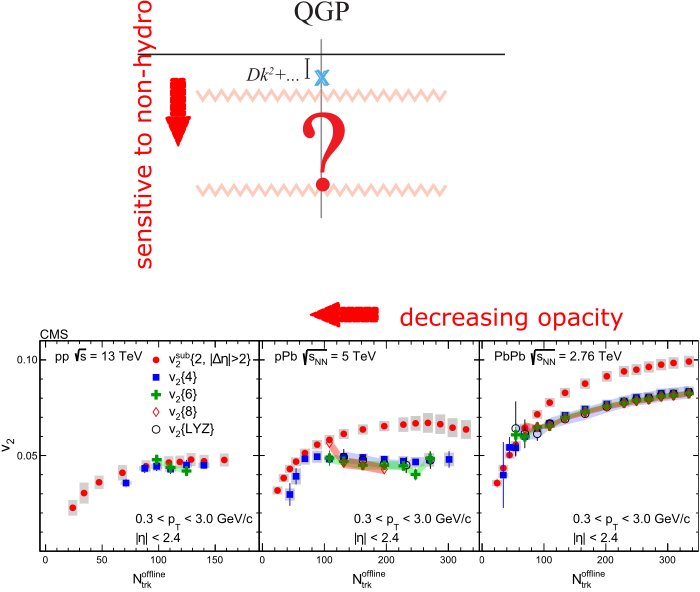
\includegraphics[width=0.6\textwidth]{fig/goal}
\end{center}
\end{frame}
%
%%%%%%%%%%%%%%%%%%%%%%%%%%%%%%%%%%%%%%%%%%%%%%%%%%%%%%%%%%
%
\begin{frame}{\bf\huge Conclusions}
\setcounter{page}{0}
\vspace{2mm}
{\color{teablue}3.} {\color{darkred}The CKT implements the same hydro as IS hydro with a physically motivated non-hydro sector. And we find}\\
\vspace{2mm}
\begin{center}
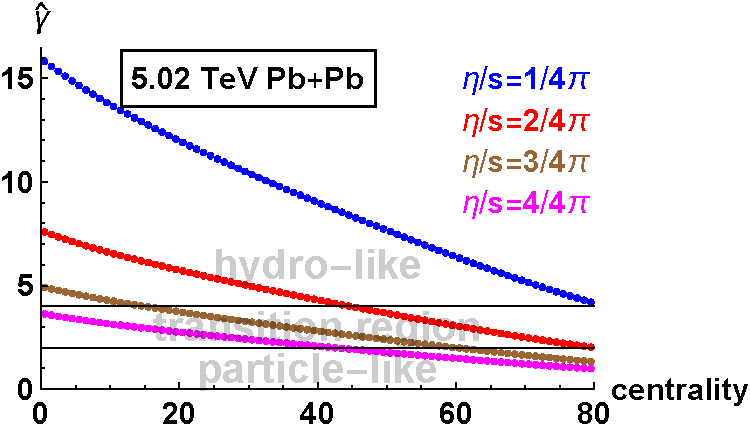
\includegraphics[width=0.4\textwidth]{fig/PbPb}\hspace{0.1\textwidth}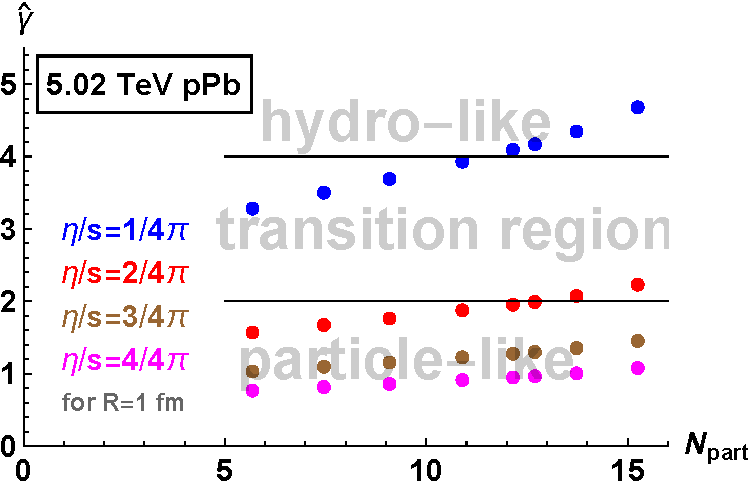
\includegraphics[width=0.4\textwidth]{fig/pPb}
\end{center}
\vspace{2mm}
And for small systems: {\color{darkred}\framebox[0.4\textwidth]{$\left.\frac{v_2}{\epsilon_2}\right|_{\hat{\gamma}<1}\propto\hat{\gamma}\propto\left( R \langle p_\perp\rangle \frac{dN}{d\eta_s}\right)^\frac{1}{4}$}
}\\
\vspace{4mm}
{\color{teablue}4.} {\color{darkred} The strategy provides a general approach \& implementation in all theories beyond hydro is most welcome.}
\end{frame}
%
%%%%%%%%%%%%%%%%%%%%%%%%%%%%%%%%%%%%%%%%%%%%%%%%%%%%%%%%%%
%
\begin{frame}
\setcounter{page}{0}
\topskip0pt
\vspace*{\fill}
\begin{center}
{\Huge\bf\color{gray}Backup Slides}
\end{center}
\vspace*{\fill}
\end{frame}
\end{document}


